\clearpage

\subsection{Opaque with 1+1 Protection}\label{heuristic_Opaque_Protection}
\begin{tcolorbox}	
\begin{tabular}{p{2.75cm} p{0.2cm} p{10.5cm}} 	
\textbf{Student Name}  &:& Pedro Coelho    (01/03/2018 - )\\
\textbf{Goal}          &:& Implement the heuristic model for the opaque transport mode with 1 plus 1 protection.
\end{tabular}
\end{tcolorbox}

\subsubsection{Model description}

The impact of failure in WDM (Wavelength Division Multiplexing) networks is caused by extremely high volume of traffic carried. In a high speed network like the WDM, a failure of a network element may cause failure of various optical channels that leads to large data and revenue losses, which can interrupt communication services.\\
In this protection scheme, the primary and backup path carry the traffic end-to-end, i.e., there is a need to have a backup path (the unaffected path) in case of a network failure. Then, the receiver will decide which one of the two incoming traffic it is going to pick, if the primary or the backup path.\\
Although it is the fastest protection scheme, it is also the most expensive, because it normally uses more than the double of the capacity of the primary path. This happens because the backup path is typically longer than the primary.\\
After the creation of the matrices and the network topology, it is necessary to apply the routing and grooming algorithms created. In the end, a report algorithm will be applied to obtain the best CAPEX result for the network in question.\\
Firstly, in the opaque transport mode, the optical node cost is 0 because all the ports in the network are electrical. Consequently, to calculate the nodes' cost in this transport mode it only has to be considered the electrical nodes' cost:

\begin{itemize}
  \item $N_{OXC,n}$ = 0, \quad $\forall$ n
  \item $N_{EXC,n}$ = 1, \quad $\forall$ n that process traffic
\end{itemize}

As previously mentioned, equation \ref{EXC_pexc1_opaque_heuristic_protec} refers to the number of long-reach ports of the electrical switch with bit-rate -1 in node $n$, $P_{exc,-1,n}$, i.e., the number of line ports of node $n$ which can be calculated as

\begin{equation}
P_{exc,-1,n} = \sum_{j=1}^{N} w_{nj}
\label{EXC_pexc1_opaque_heuristic_protec}
\end{equation}

\noindent
where $w_{nj}$ is the number of optical channels between node $n$ and node $j$.

\newpage
\vspace{11pt}
As previously mentioned, equation \ref{EXC_pexc2_opaque_heuristic_protec} refers to the number of short-reach ports of the electrical switch with bit-rate $c$ in node $n$, $P_{exc,c,n}$, i.e., the number of tributary ports with bit-rate $c$ in node $n$ which can be calculated as

\begin{equation}
P_{exc,c,n} = \sum_{d=1}^{N} D_{nd,c}
\label{EXC_pexc2_opaque_heuristic_protec}
\end{equation}

\noindent
where $D_{nd,c}$ are the client demands between nodes $n$ and $d$ with bit rate $c$.\\

\noindent
In this case there is the following particularity:

\begin{itemize}
  \item When $n$=$j$, the value of client demands is always zero, i.e, $D_{nn,c}=0$.
\end{itemize}

\noindent
The function, to be minimized, is the expression \ref{Minimize_Heuristic_CAPEX}.\\

\subsubsection{Result description}

It is already known all the necessary formulas to obtain the CAPEX value for the reference network \ref{Reference_Network_Topology}. As described in the subsection of the network traffic \ref{Reference_Network_Traffic}, it is necessary to obtain three different values of CAPEX for the low (0.5 Tbit/s), medium (5 Tbit/s) and high (10 Tbit/s) traffic. It is used a network software program called Net2Plan which can design the traffic matrices, create all the network topologies, simulate the algorithms into the network implemented in the programming software called Eclipse and analyze the results obtained.\\
In this chapter will be demonstrated the results by Vasco's heuristics from 2016. In each of the three traffic scenarios, it will be shown the network topologies followed by the table with the CAPEX value of the network.\\

\textbf{Low Traffic Scenario:}\\

In this scenario we have to take into account the traffic calculated in \ref{low_scenario}. In a first phase we will show the various existing topologies of the network. The first are the allowed topologies, physical and optical topologies, the second are the logical topology for all ODUs and finally the resulting physical topology.\\

\begin{figure}[H]
\centering
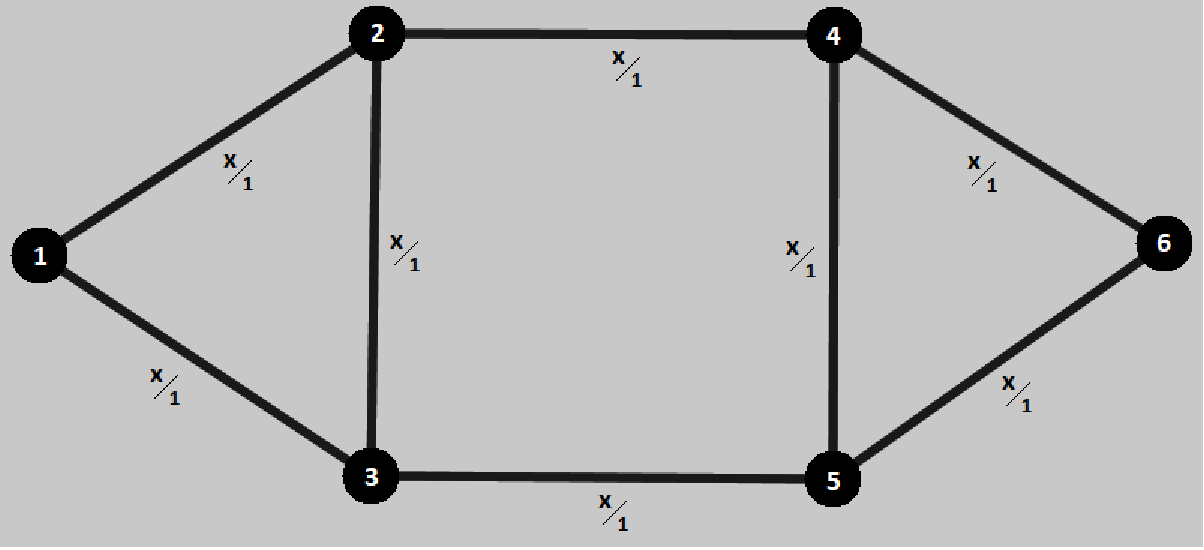
\includegraphics[width=13cm]{sdf/heuristic/opaque_protection/figures/allowed_physical}
\caption{Allowed physical topology. The allowed physical topology is defined by the duct and sites in the field. It is assumed that each duct supports up to 1 bidirectional transmission system and each site supports up to 1 node.}
\label{allowed_physical_protec_ref_low_heuristic}
\end{figure}

\begin{figure}[H]
\centering
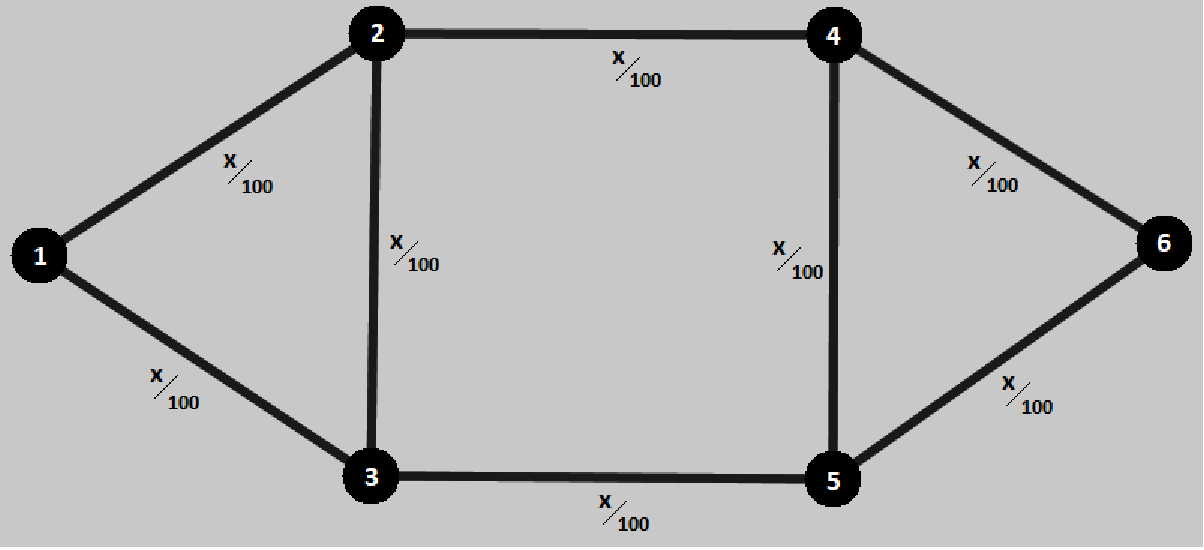
\includegraphics[width=13cm]{sdf/heuristic/opaque_protection/figures/allowed_optical}
\caption{Allowed optical topology. The allowed optical topology is defined by the transport mode (opaque transport mode in this case). It is assumed that each transmission system supports up to 100 optical channels.}
\label{allowed_optical_protec_ref_low_heuristic}
\end{figure}

\begin{figure}[H]
\centering
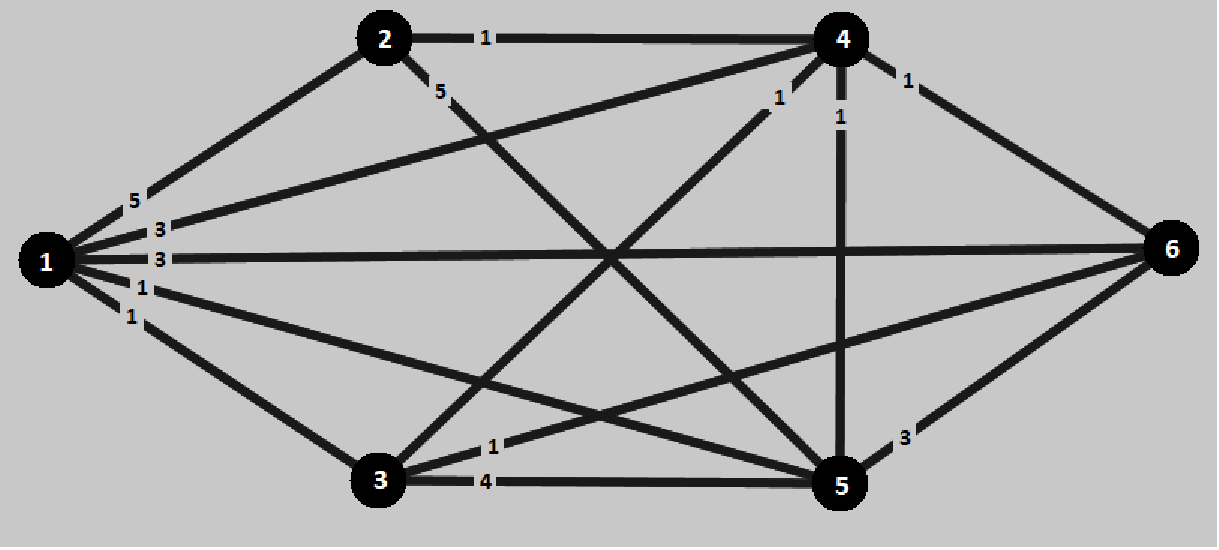
\includegraphics[width=13cm]{sdf/heuristic/opaque_protection/figures/logical_topology_odu0_low}
\caption{ODU0 logical topology defined by the ODU0 traffic matrix.}
\label{logical_ODU0_protec_ref_low_heuristic}
\end{figure}

\begin{figure}[H]
\centering
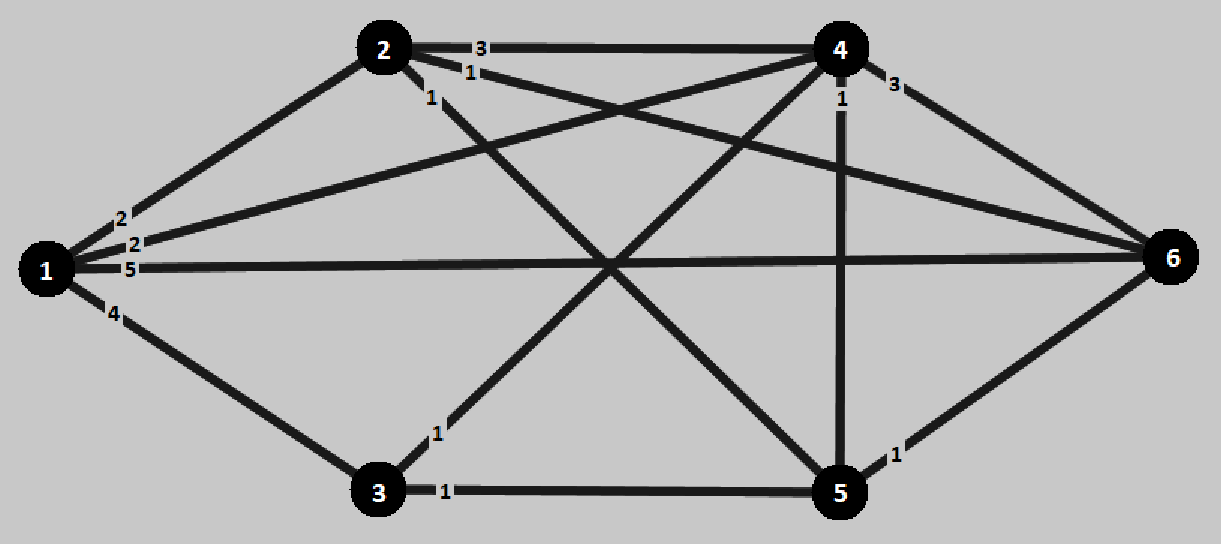
\includegraphics[width=13cm]{sdf/heuristic/opaque_protection/figures/logical_topology_odu1_low}
\caption{ODU1 logical topology defined by the ODU1 traffic matrix.}
\label{logical_ODU1_protec_ref_low_heuristic}
\end{figure}

\begin{figure}[H]
\centering
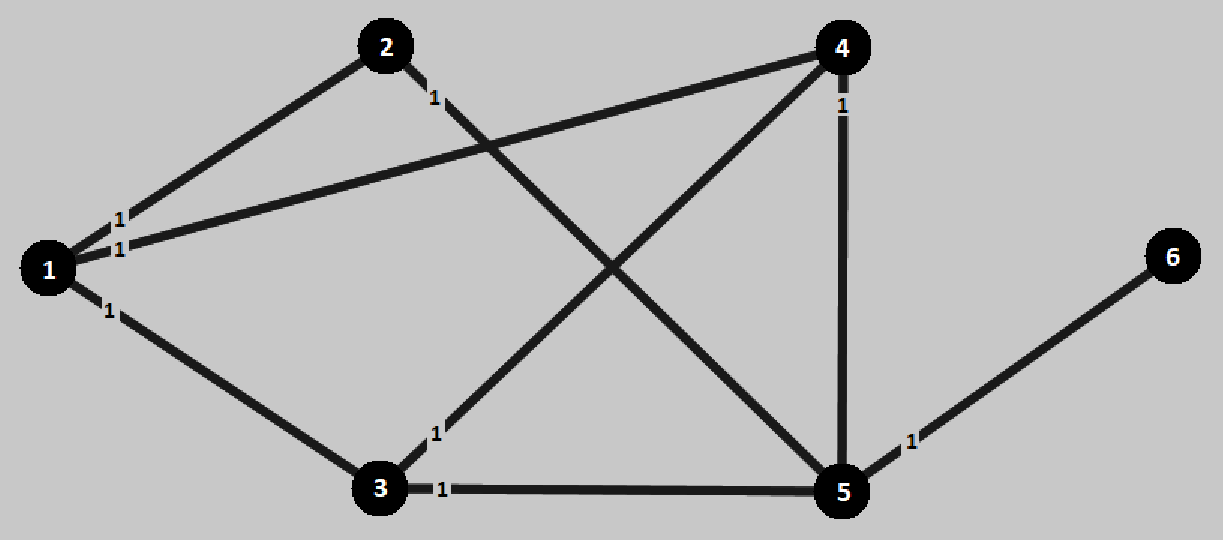
\includegraphics[width=13cm]{sdf/heuristic/opaque_protection/figures/logical_topology_odu2_low}
\caption{ODU2 logical topology defined by the ODU2 traffic matrix.}
\label{logical_ODU2_protec_ref_low_heuristic}
\end{figure}

\begin{figure}[H]
\centering
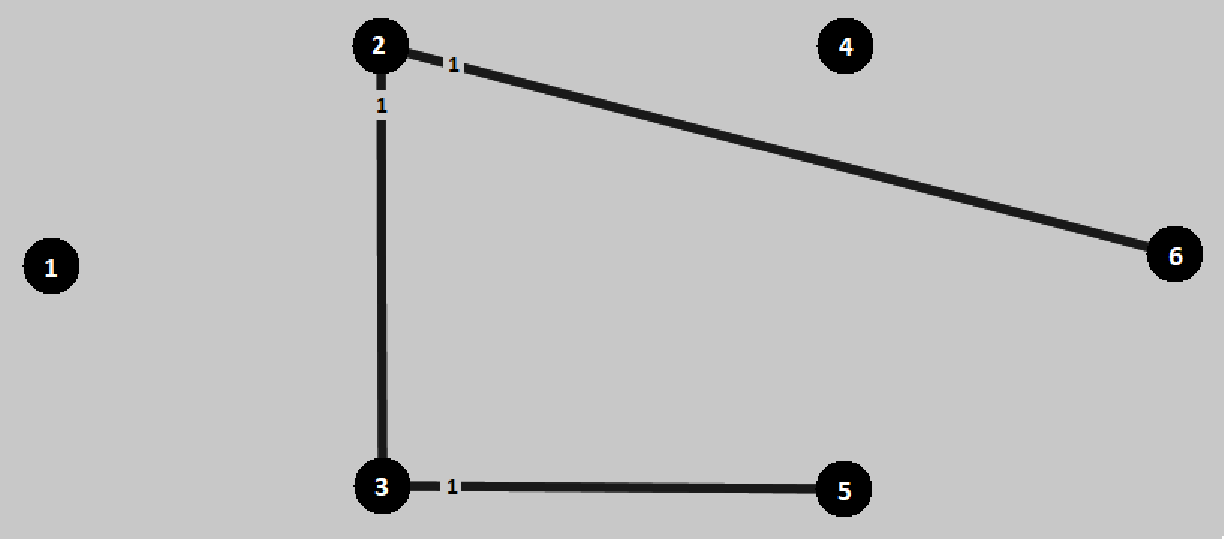
\includegraphics[width=13cm]{sdf/heuristic/opaque_protection/figures/logical_topology_odu3_low}
\caption{ODU3 logical topology defined by the ODU3 traffic matrix.}
\label{logical_ODU3_protec_ref_low_heuristic}
\end{figure}

\begin{figure}[H]
\centering
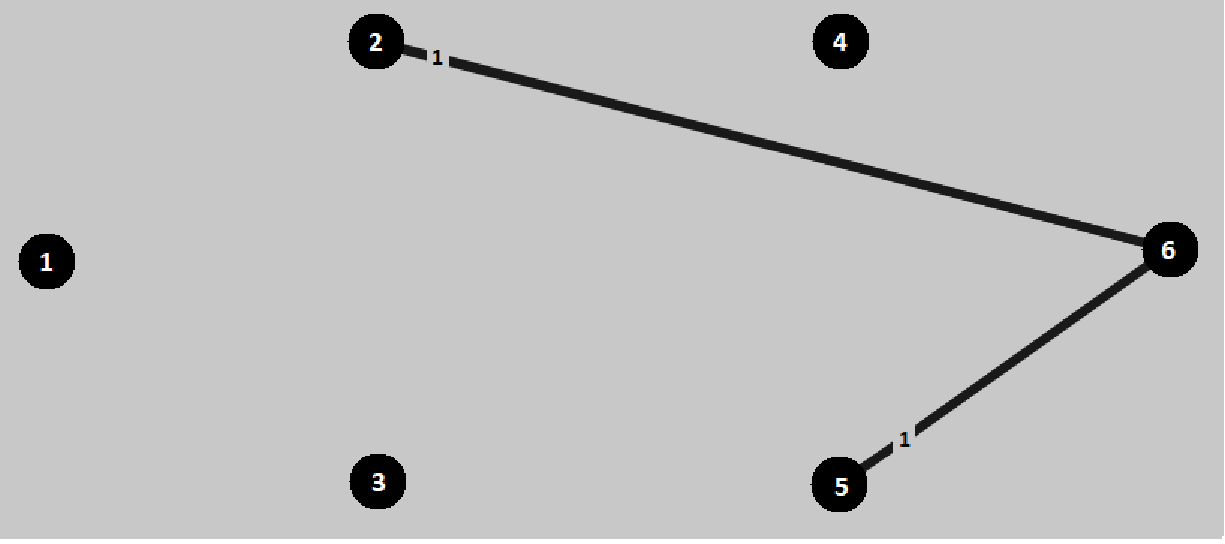
\includegraphics[width=13cm]{sdf/heuristic/opaque_protection/figures/logical_topology_odu4_low}
\caption{ODU4 logical topology defined by the ODU4 traffic matrix.}
\label{logical_ODU4_protec_ref_low_heuristic}
\end{figure}

\begin{figure}[H]
\centering
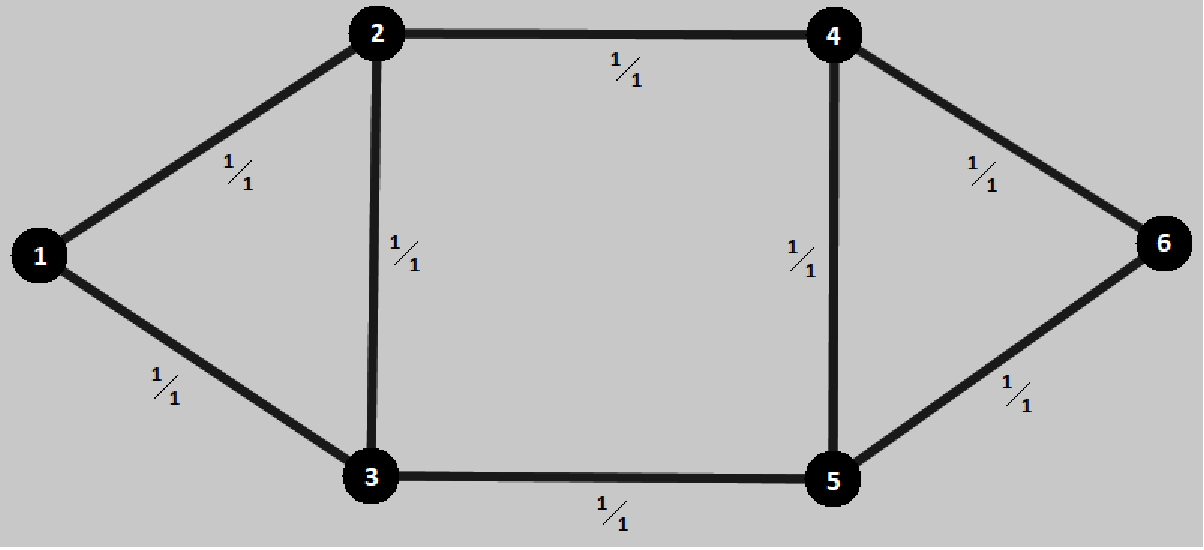
\includegraphics[width=13cm]{sdf/heuristic/opaque_protection/figures/physical_topology}
\caption{Physical topology after dimensioning.}
\label{physical_topology_protec_ref_low_heuristic}
\end{figure}

\begin{figure}[H]
\centering
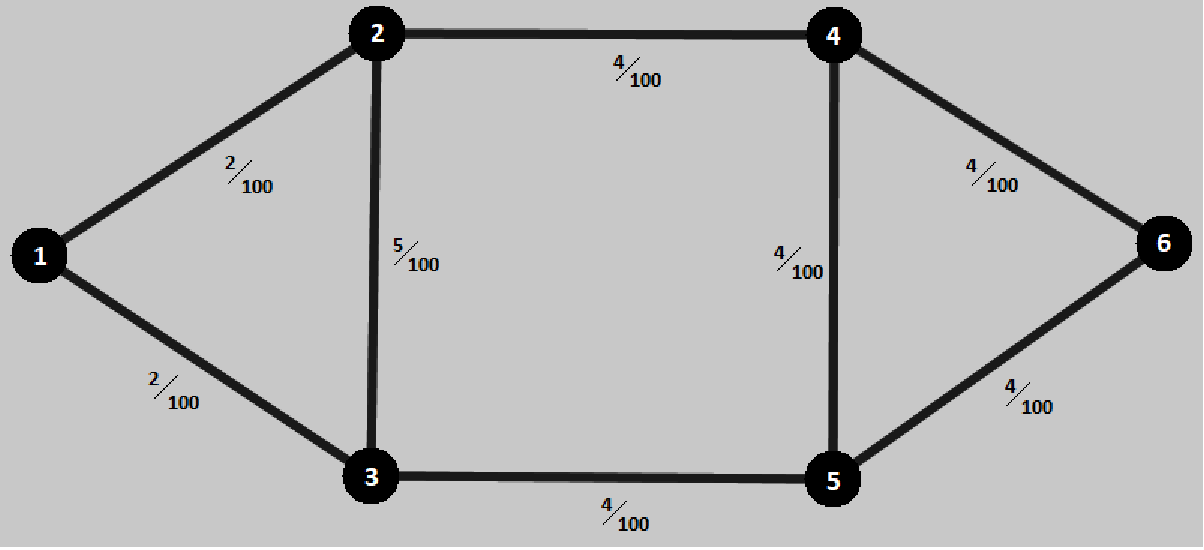
\includegraphics[width=13cm]{sdf/heuristic/opaque_protection/figures/optical_topology_low}
\caption{Optical topology after dimensioning.}
\label{optical_topology_protec_ref_low_heuristic}
\end{figure}

Following all the steps mentioned in the \ref{net2plan_guide}, applying the routing and grooming heuristic algorithms in the Net2Plan software and using all the data referring to this scenario, the obtained result for the Vasco's heuristics can be consulted in the following table \ref{scriptopaque_protec_ref_low_heuristic}. In table \ref{formulas_opaque_heuristic} mentioned in previous model we can see how all the values were calculated. \\

\begin{table}[H]
\centering
\begin{tabular}{|| c | c | c | c | c | c | c ||}
 \hline
 \multicolumn{7}{|| c ||}{CAPEX of the Network} \\
 \hline
 \hline
 \multicolumn{3}{|| c |}{ } & Quantity & Unit Price & Cost & Total \\
 \hline
 \multirow{3}{*}{\makecell{Link \\ Cost}} & \multicolumn{2}{ c |}{OLTs} & 16 & 15 000 \euro & 240 000 \euro & \multirow{3}{*}{23 520 000 \euro} \\ \cline{2-6}
 & \multicolumn{2}{ c |}{100 Gbits/s Transceivers} & 46 & 5 000 \euro/Gbit/s & 23 000 000 \euro & \\ \cline{2-6}
 & \multicolumn{2}{ c |}{Amplifiers} & 70 & 4 000 \euro & 280 000 \euro & \\
 \hline
 \multirow{9}{*}{\makecell{Node \\ Cost}} & \multirow{7}{*}{Electrical} & EXCs & 6 & 10 000 \euro & 60 000 \euro & \multirow{9}{*}{4 662 590 \euro} \\ \cline{3-6}
  & & ODU0 Ports & 60 & 10 \euro/port & 600 \euro & \\ \cline{3-6}
 & & ODU1 Ports & 50 & 15 \euro/port & 750 \euro & \\ \cline{3-6}
 & & ODU2 Ports & 16 & 30 \euro/port & 480 \euro & \\ \cline{3-6}
 & & ODU3 Ports & 6 & 60 \euro/port & 360 \euro & \\ \cline{3-6}
 & & ODU4 Ports & 4 & 100 \euro/port & 400 \euro & \\ \cline{3-6}
 & & Line Ports & 46 & 100 000 \euro/port & 4 600 000 \euro & \\ \cline{2-6}
 & \multirow{2}{*}{Optical} & OXCs & 0 & 20 000 \euro & 0 \euro & \\ \cline{3-6}
 & & Ports & 0 & 2 500 \euro/port & 0 \euro & \\
 \hline
 \multicolumn{6}{|| c |}{Total Network Cost} & 28 182 590 \euro \\
\hline
\end{tabular}
\caption{Table with detailed description of CAPEX of Vasco's 2016 results.}
\label{scriptopaque_protec_ref_low_heuristic}
\end{table}

\newpage
\textbf{Medium Traffic Scenario:}\\

In this scenario we have to take into account the traffic calculated in \ref{medium_traffic_scenario}. In a first phase we will show the various existing topologies of the network. The first are the allowed topologies, physical and optical topologies, the second are the logical topology for all ODUs and finally the resulting physical topology.\\

\begin{figure}[H]
\centering
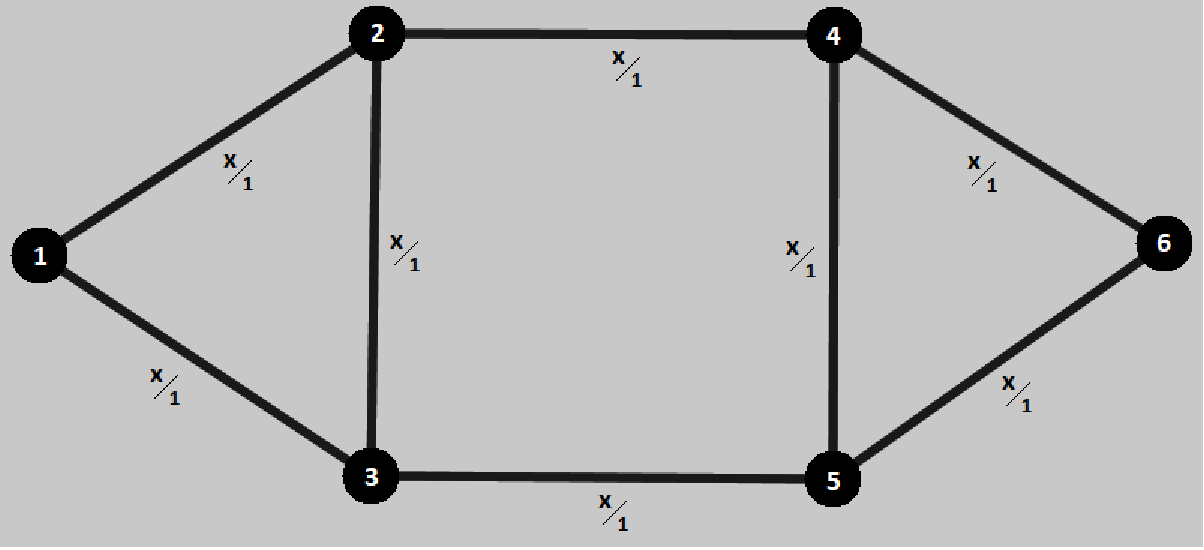
\includegraphics[width=13cm]{sdf/heuristic/opaque_protection/figures/allowed_physical}
\caption{Allowed physical topology. The allowed physical topology is defined by the duct and sites in the field. It is assumed that each duct supports up to 1 bidirectional transmission system and each site supports up to 1 node.}
\label{allowed_physical_protec_ref_medium_heuristic}
\end{figure}

\begin{figure}[H]
\centering
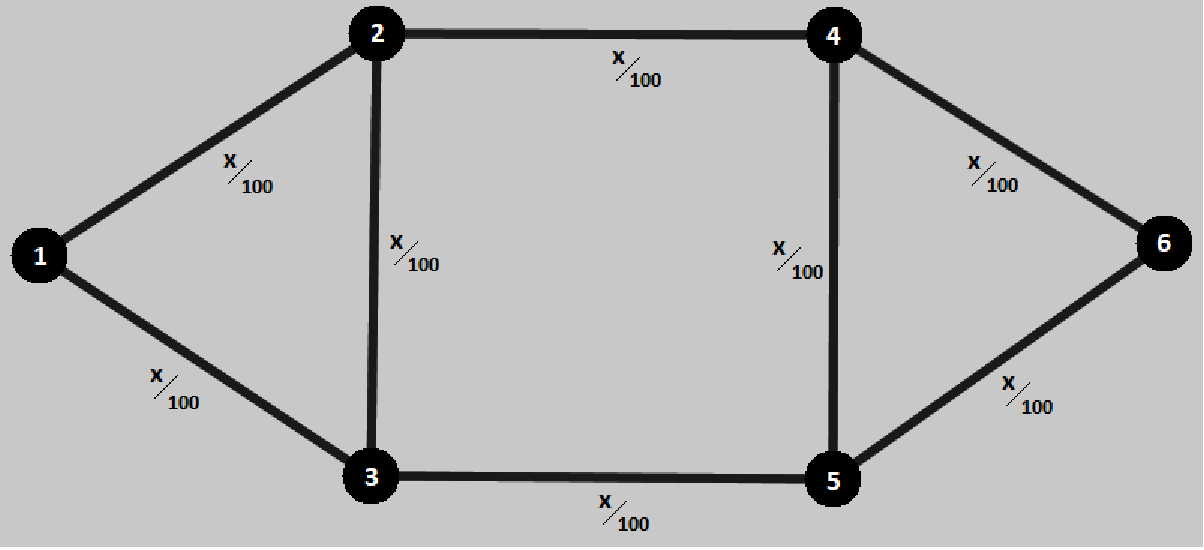
\includegraphics[width=13cm]{sdf/heuristic/opaque_protection/figures/allowed_optical}
\caption{Allowed optical topology. The allowed optical topology is defined by the transport mode (opaque transport mode in this case). It is assumed that each transmission system supports up to 100 optical channels.}
\label{allowed_optical_protec_ref_medium_heuristic}
\end{figure}

\begin{figure}[H]
\centering
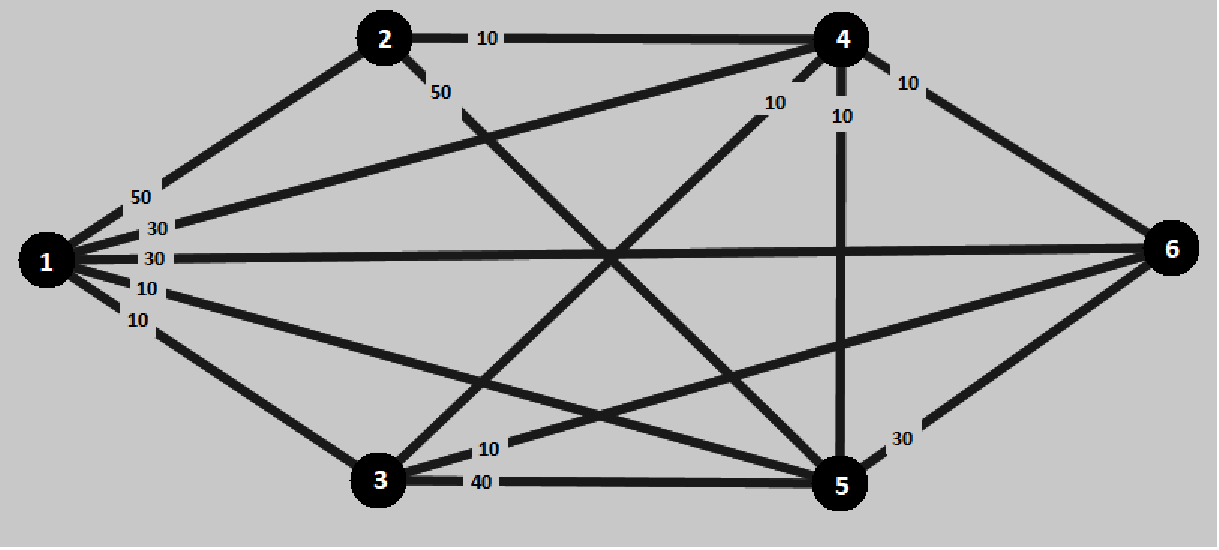
\includegraphics[width=13cm]{sdf/heuristic/opaque_protection/figures/logical_topology_odu0_medium}
\caption{ODU0 logical topology defined by the ODU0 traffic matrix.}
\label{logical_ODU0_protec_ref_medium_heuristic}
\end{figure}

\begin{figure}[H]
\centering
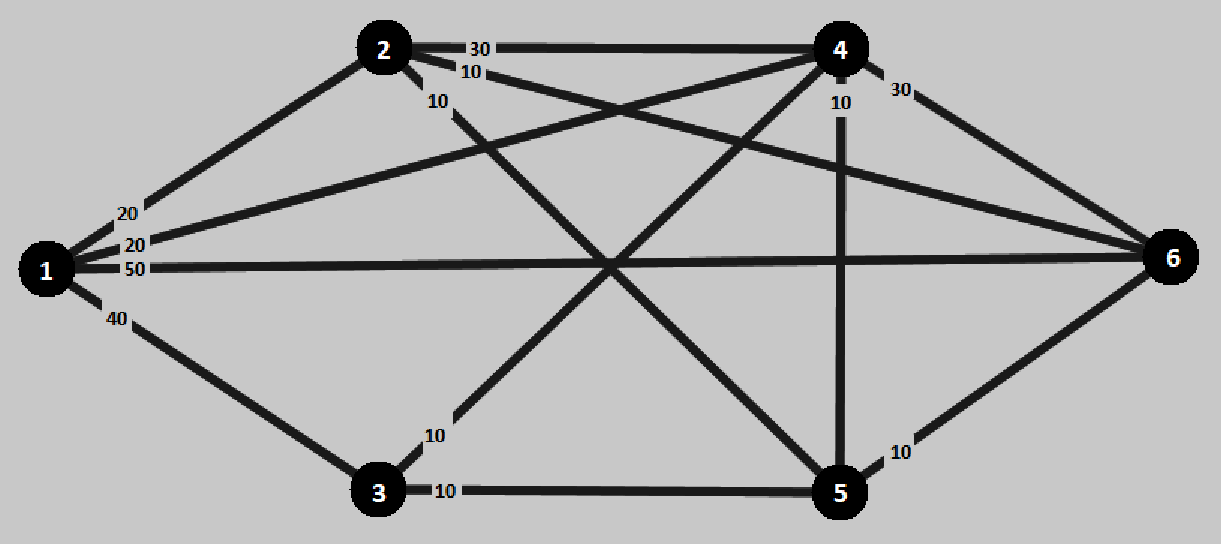
\includegraphics[width=13cm]{sdf/heuristic/opaque_protection/figures/logical_topology_odu1_medium}
\caption{ODU1 logical topology defined by the ODU1 traffic matrix.}
\label{logical_ODU1_protec_ref_medium_heuristic}
\end{figure}

\begin{figure}[H]
\centering
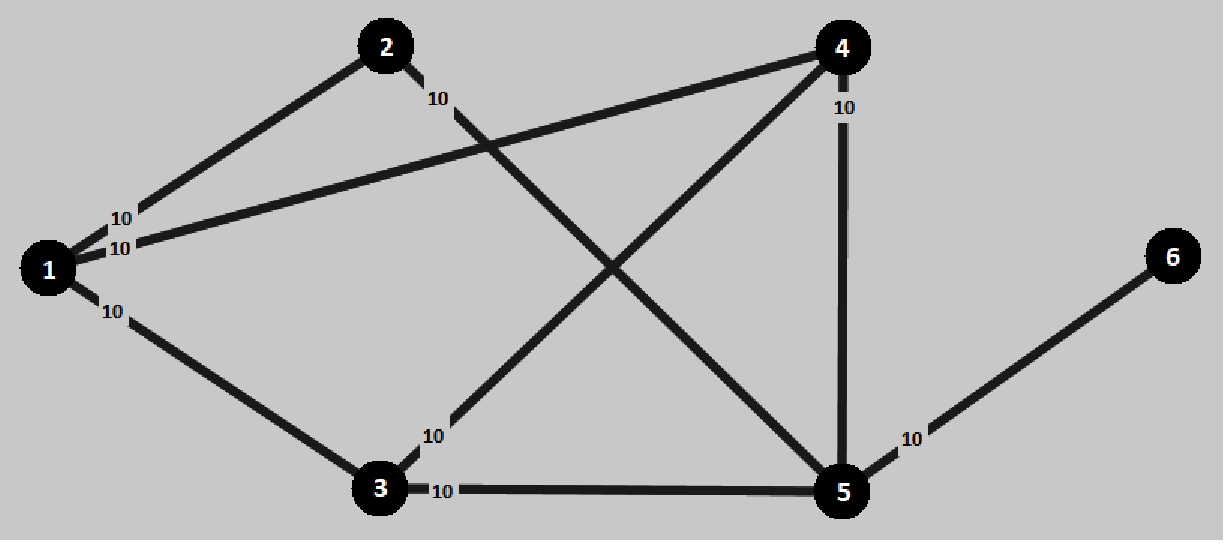
\includegraphics[width=13cm]{sdf/heuristic/opaque_protection/figures/logical_topology_odu2_medium}
\caption{ODU2 logical topology defined by the ODU2 traffic matrix.}
\label{logical_ODU2_protec_ref_medium_heuristic}
\end{figure}

\begin{figure}[H]
\centering
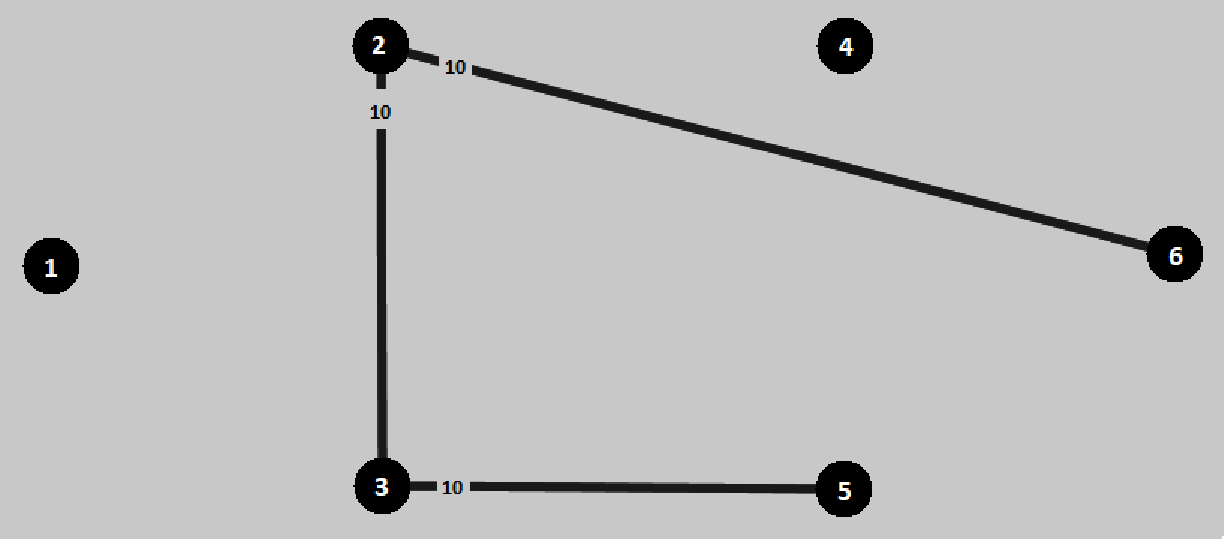
\includegraphics[width=13cm]{sdf/heuristic/opaque_protection/figures/logical_topology_odu3_medium}
\caption{ODU03 logical topology defined by the ODU3 traffic matrix.}
\label{logical_ODU3_protec_ref_medium_heuristic}
\end{figure}

\begin{figure}[H]
\centering
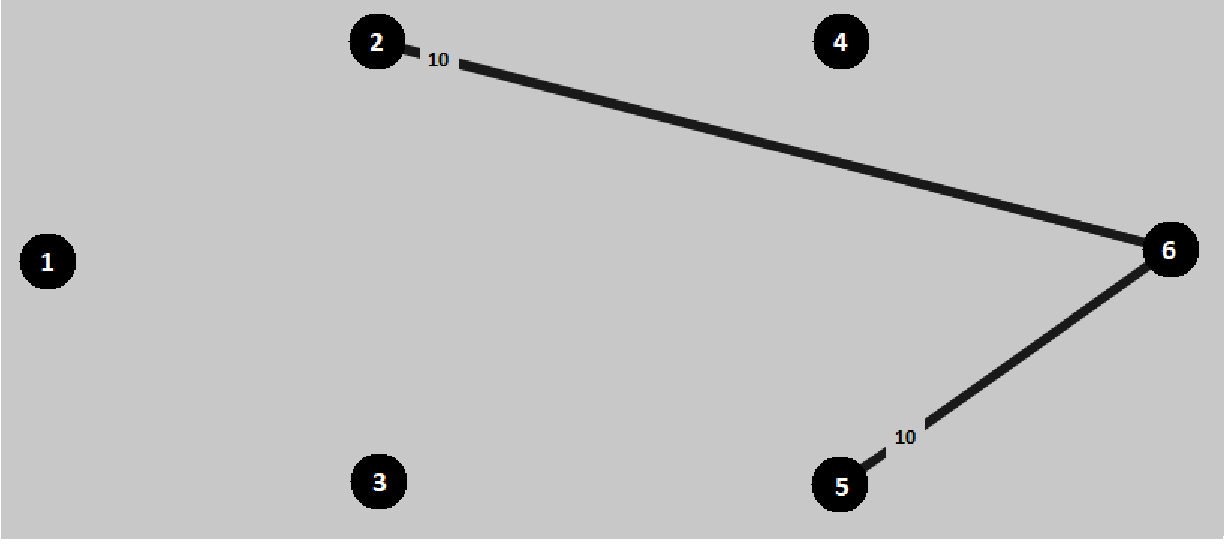
\includegraphics[width=13cm]{sdf/heuristic/opaque_protection/figures/logical_topology_odu4_medium}
\caption{ODU4 logical topology defined by the ODU4 traffic matrix.}
\label{logical_ODU4_protec_ref_medium_heuristic}
\end{figure}

\begin{figure}[H]
\centering
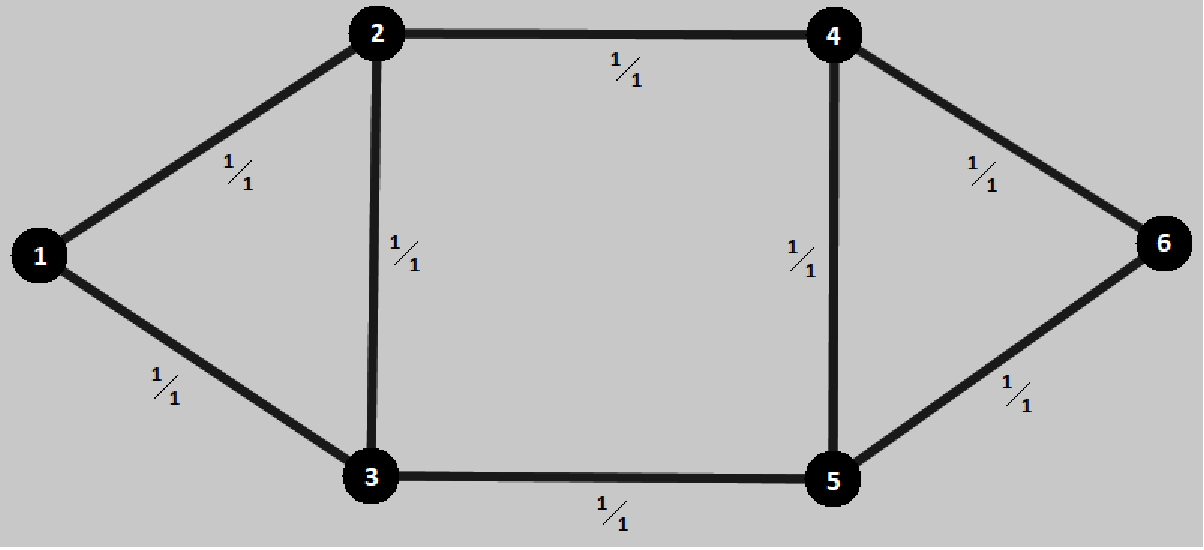
\includegraphics[width=13cm]{sdf/heuristic/opaque_protection/figures/physical_topology}
\caption{Physical topology after dimensioning.}
\label{physical_topology_protec_ref_medium_heuristic}
\end{figure}

\begin{figure}[H]
\centering
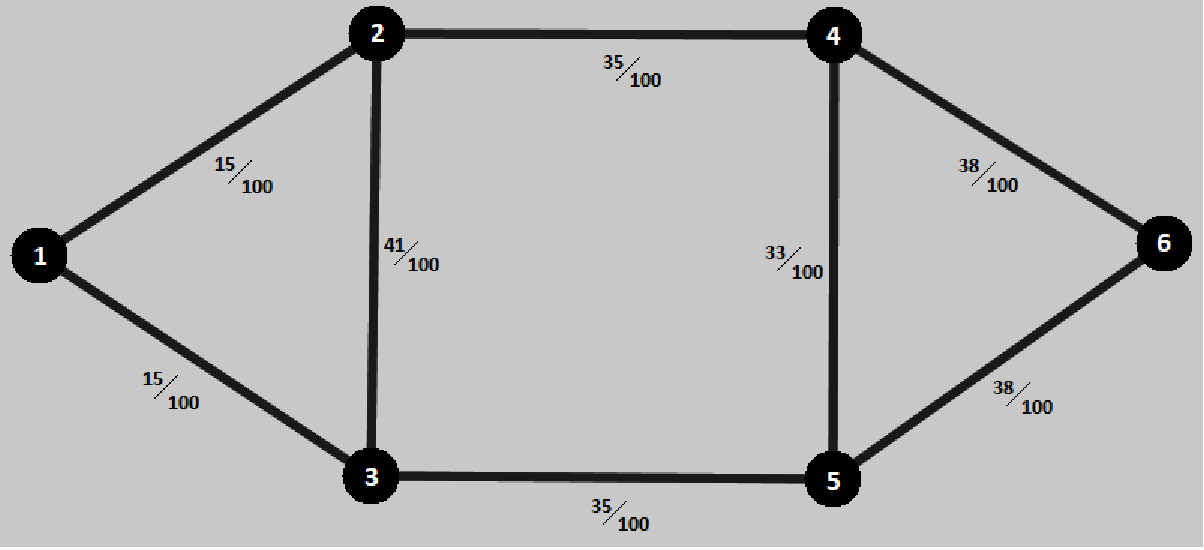
\includegraphics[width=13cm]{sdf/heuristic/opaque_protection/figures/optical_topology_medium}
\caption{Optical topology after dimensioning.}
\label{optical_topology_protec_ref_medium_heuristic}
\end{figure}

Following all the steps mentioned in the \ref{net2plan_guide}, applying the routing and grooming heuristic algorithms in the Net2Plan software and using all the data referring to this scenario, the obtained result for the Vasco's heuristics can be consulted in the following table \ref{scriptopaque_protec_ref_medium_heuristic}. In table \ref{formulas_opaque_heuristic} mentioned in previous model we can see how all the values were calculated. \\

\begin{table}[H]
\centering
\begin{tabular}{|| c | c | c | c | c | c | c ||}
 \hline
 \multicolumn{7}{|| c ||}{CAPEX of the Network} \\
 \hline
 \hline
 \multicolumn{3}{|| c |}{ } & Quantity & Unit Price & Cost & Total \\
 \hline
 \multirow{3}{*}{\makecell{Link \\ Cost}} & \multicolumn{2}{ c |}{OLTs} & 16 & 15 000 \euro & 240 000 \euro & \multirow{3}{*}{199 520 000 \euro} \\ \cline{2-6}
 & \multicolumn{2}{ c |}{100 Gbits/s Transceivers} & 398 & 5 000 \euro/Gbit/s & 199 000 000 \euro & \\ \cline{2-6}
 & \multicolumn{2}{ c |}{Amplifiers} & 70 & 4 000 \euro & 280 000 \euro & \\
 \hline
 \multirow{9}{*}{\makecell{Node \\ Cost}} & \multirow{7}{*}{Electrical} & EXCs & 6 & 10 000 \euro & 60 000 \euro & \multirow{9}{*}{39 885 900 \euro} \\ \cline{3-6}
 & & ODU0 Ports & 600 & 10 \euro/port & 6 000 \euro & \\ \cline{3-6}
 & & ODU1 Ports & 500 & 15 \euro/port & 7 500 \euro & \\ \cline{3-6}
 & & ODU2 Ports & 160 & 30 \euro/port & 4 800 \euro & \\ \cline{3-6}
 & & ODU3 Ports & 60 & 60 \euro/port & 3 600 \euro & \\ \cline{3-6}
 & & ODU4 Ports & 40 & 100 \euro/port & 4 000 \euro & \\ \cline{3-6}
 & & Line Ports & 398 & 100 000 \euro/port & 50 000 000 \euro & \\ \cline{2-6}
 & \multirow{2}{*}{Optical} & OXCs & 0 & 20 000 \euro & 0 \euro & \\ \cline{3-6}
 & & Ports & 0 & 2 500 \euro/port & 0 \euro & \\
 \hline
 \multicolumn{6}{|| c |}{Total Network Cost} & 239 405 900 \euro \\
\hline
\end{tabular}
\caption{Table with detailed description of CAPEX of Vasco's 2016 results.}
\label{scriptopaque_protec_ref_medium_heuristic}
\end{table}

\textbf{High Traffic Scenario:}\\

In this scenario we have to take into account the traffic calculated in \ref{high_traffic_scenario}. In a first phase we will show the various existing topologies of the network. The first are the allowed topologies, physical and optical topologies, the second are the logical topology for all ODUs and finally the resulting physical topology.\\

\begin{figure}[H]
\centering
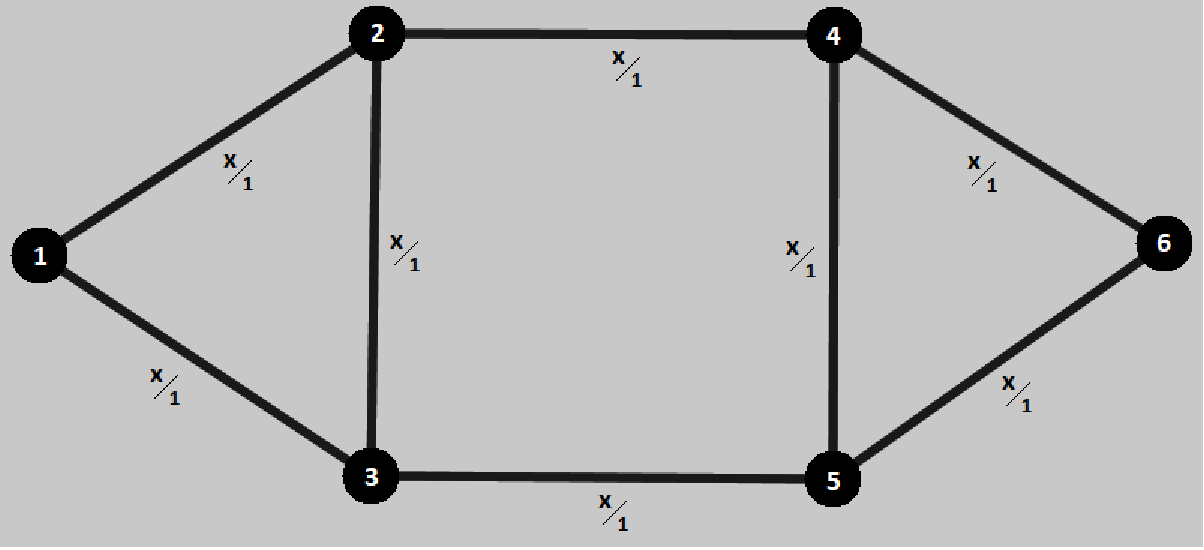
\includegraphics[width=13cm]{sdf/heuristic/opaque_protection/figures/allowed_physical}
\caption{Allowed physical topology. The allowed physical topology is defined by the duct and sites in the field. It is assumed that each duct supports up to 1 bidirectional transmission system and each site supports up to 1 node.}
\label{allowed_physical_protec_ref_high_heuristic}
\end{figure}

\begin{figure}[H]
\centering
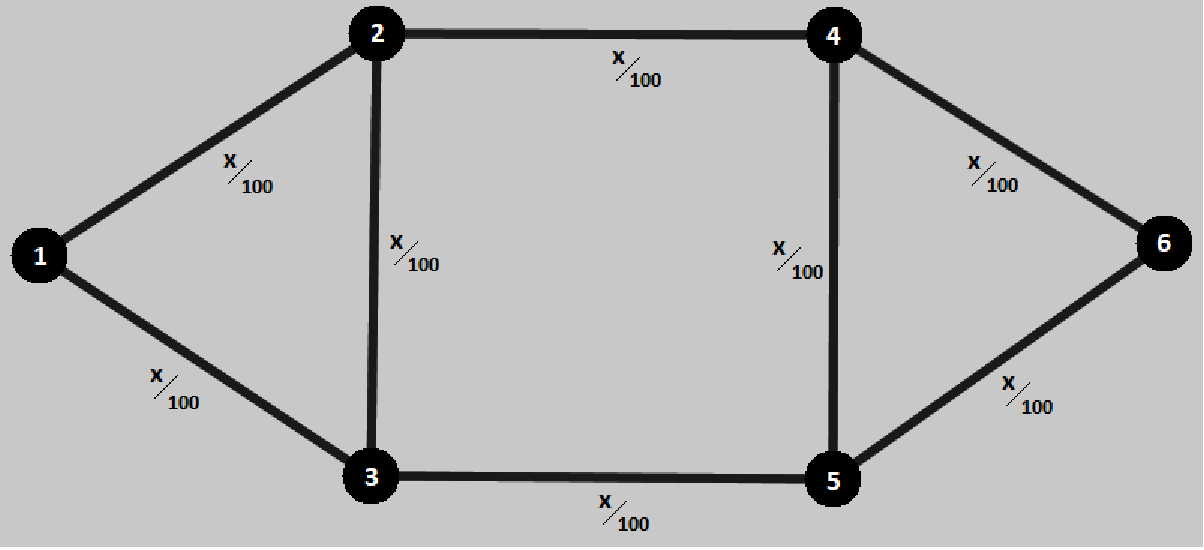
\includegraphics[width=13cm]{sdf/heuristic/opaque_protection/figures/allowed_optical}
\caption{Allowed optical topology. The allowed optical topology is defined by the transport mode (opaque transport mode in this case). It is assumed that each transmission system supports up to 100 optical channels.}
\label{allowed_optical_protec_ref_high_heuristic}
\end{figure}

\begin{figure}[H]
\centering
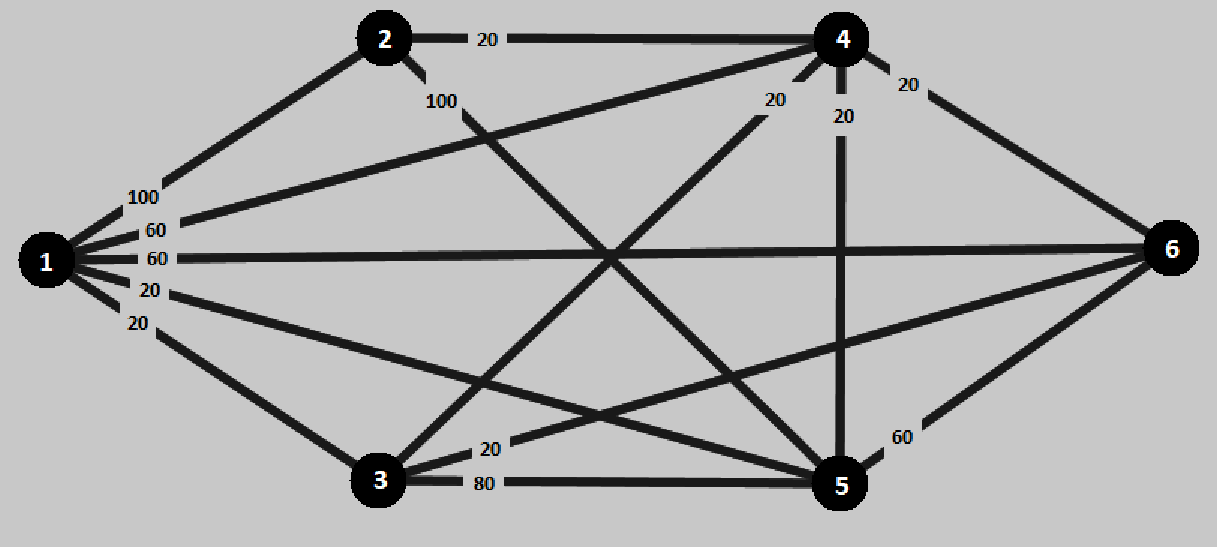
\includegraphics[width=13cm]{sdf/heuristic/opaque_protection/figures/logical_topology_odu0_high}
\caption{ODU0 logical topology defined by the ODU0 traffic matrix.}
\label{logical_ODU0_protec_ref_high_heuristic}
\end{figure}

\begin{figure}[H]
\centering
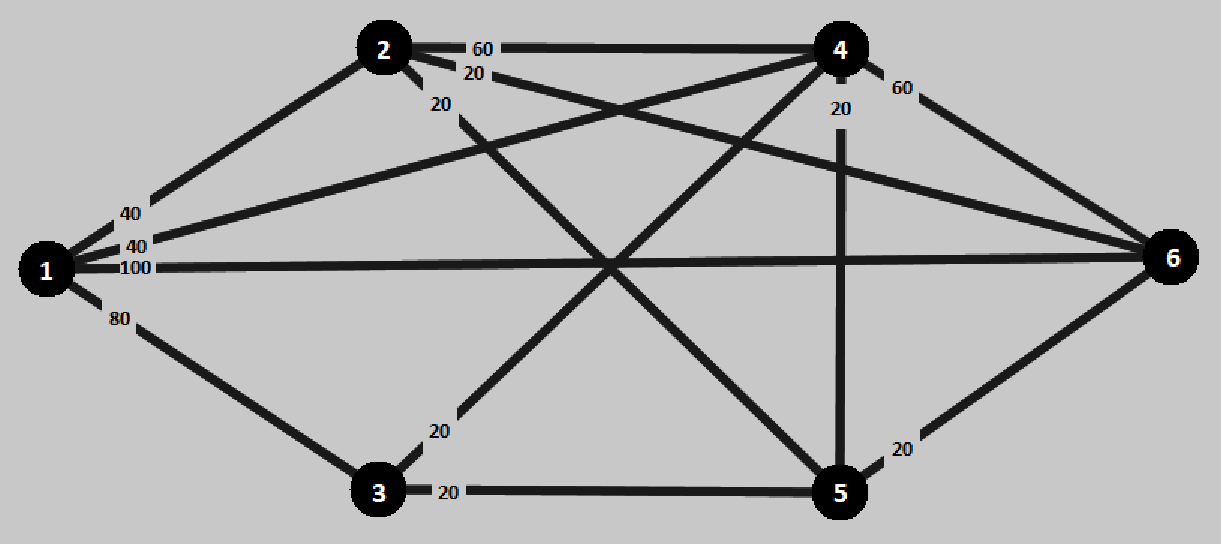
\includegraphics[width=13cm]{sdf/heuristic/opaque_protection/figures/logical_topology_odu1_high}
\caption{ODU1 logical topology defined by the ODU1 traffic matrix.}
\label{logical_ODU1_protec_ref_high_heuristic}
\end{figure}

\begin{figure}[H]
\centering
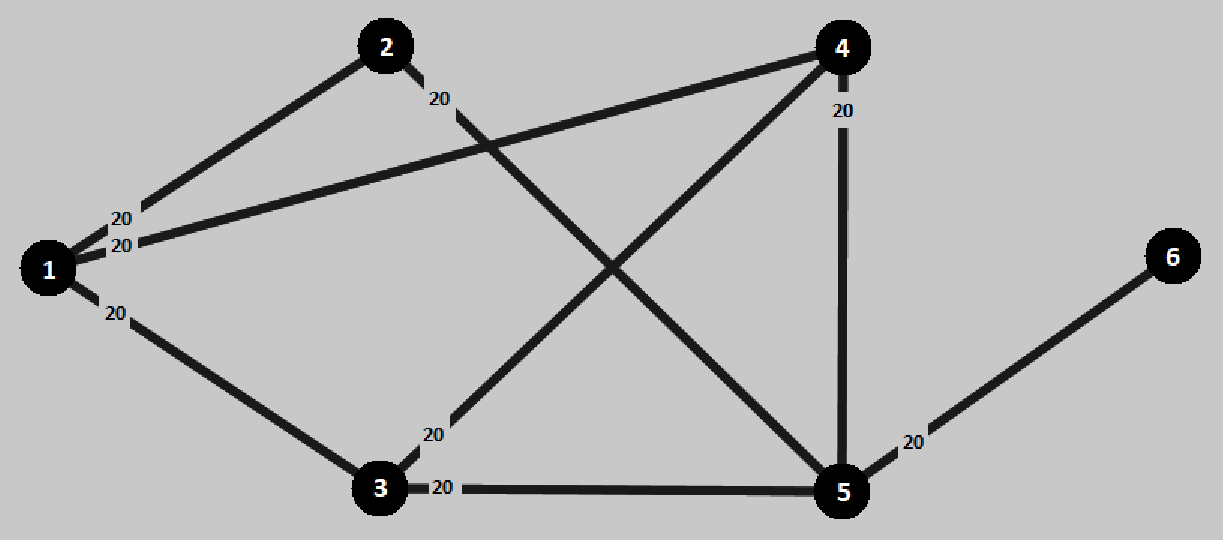
\includegraphics[width=13cm]{sdf/heuristic/opaque_protection/figures/logical_topology_odu2_high}
\caption{ODU2 logical topology defined by the ODU2 traffic matrix.}
\label{logical_ODU2_protec_ref_high_heuristic}
\end{figure}

\begin{figure}[H]
\centering
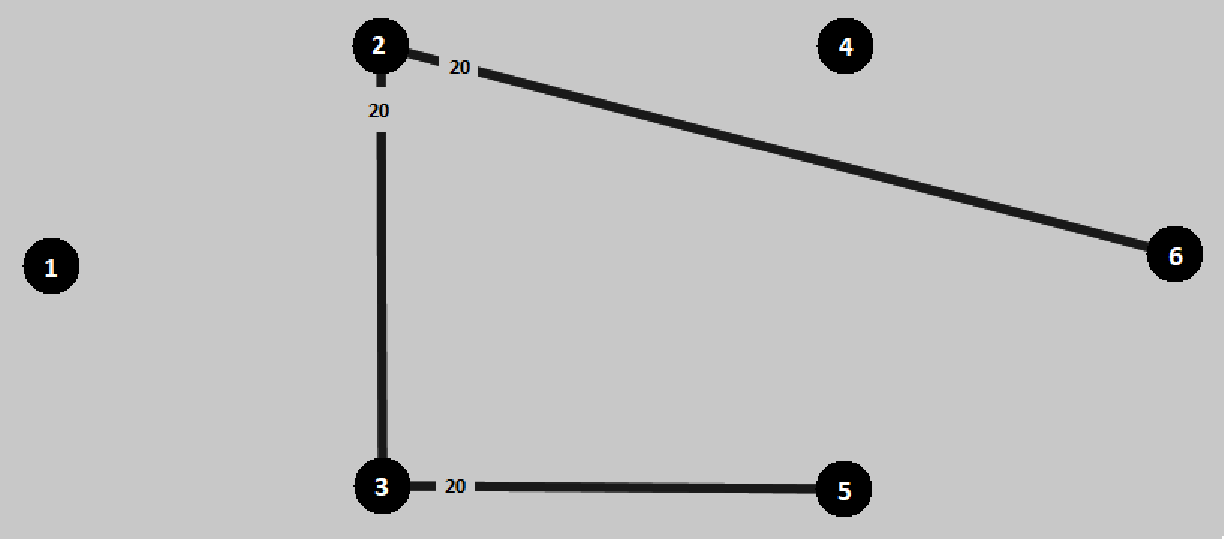
\includegraphics[width=13cm]{sdf/heuristic/opaque_protection/figures/logical_topology_odu3_high}
\caption{ODU3 logical topology defined by the ODU3 traffic matrix.}
\label{logical_ODU3_protec_ref_high_heuristic}
\end{figure}

\begin{figure}[H]
\centering
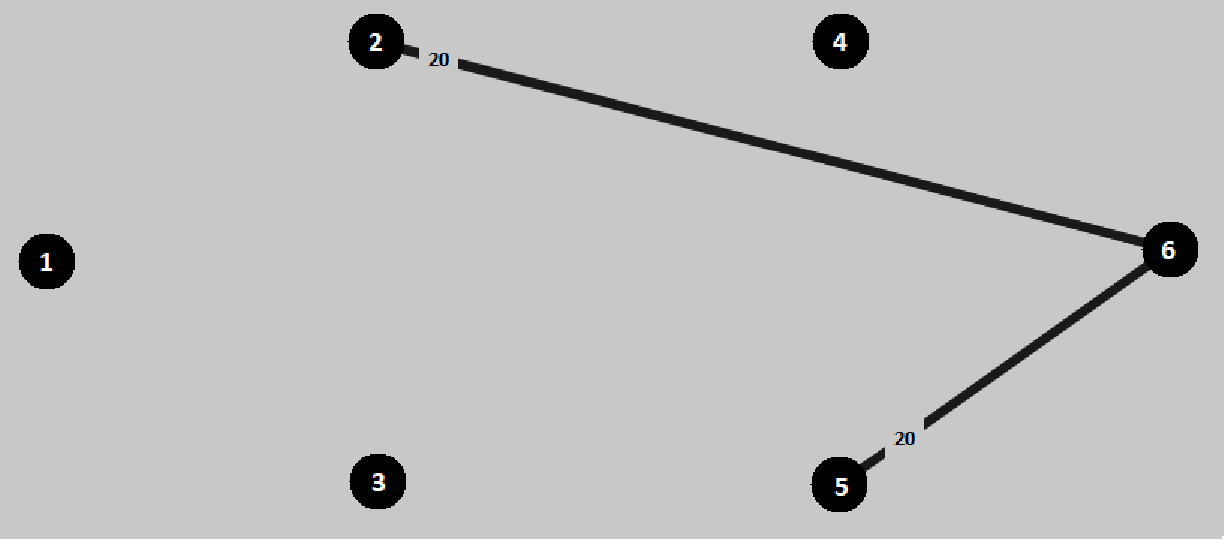
\includegraphics[width=13cm]{sdf/heuristic/opaque_protection/figures/logical_topology_odu4_high}
\caption{ODU4 logical topology defined by the ODU4 traffic matrix.}
\label{logical_ODU4_protec_ref_high_heuristic}
\end{figure}

\begin{figure}[H]
\centering
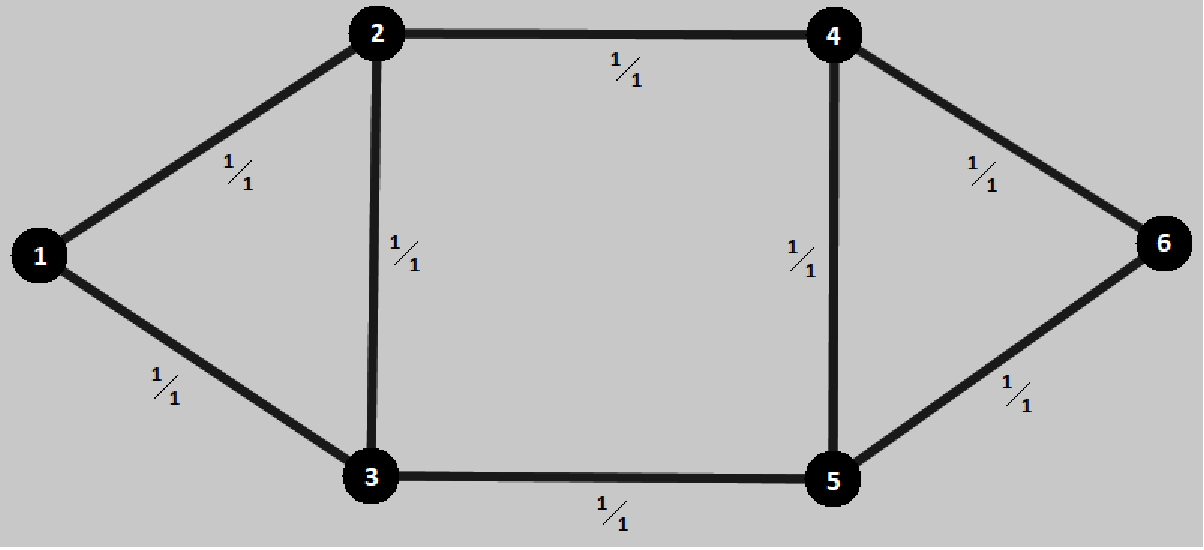
\includegraphics[width=13cm]{sdf/heuristic/opaque_protection/figures/physical_topology}
\caption{Physical topology after dimensioning.}
\label{physical_topology_protec_ref_high_heuristic}
\end{figure}

\begin{figure}[H]
\centering
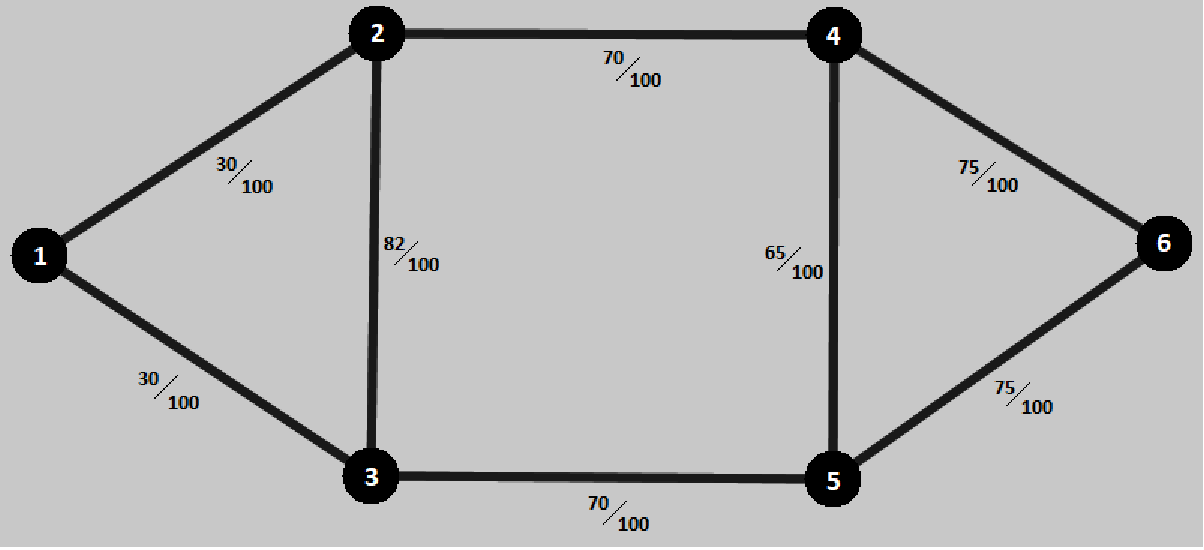
\includegraphics[width=13cm]{sdf/heuristic/opaque_protection/figures/optical_topology_high}
\caption{Optical topology after dimensioning.}
\label{optical_topology_protec_ref_high_heuristic}
\end{figure}

Following all the steps mentioned in the \ref{net2plan_guide}, applying the routing and grooming heuristic algorithms in the Net2Plan software and using all the data referring to this scenario, the obtained result for the Vasco's heuristics can be consulted in the following table \ref{scriptopaque_protec_ref_high_heuristic}. In table \ref{formulas_opaque_heuristic} mentioned in previous model we can see how all the values were calculated. \\

\begin{table}[H]
\centering
\begin{tabular}{|| c | c | c | c | c | c | c ||}
 \hline
 \multicolumn{7}{|| c ||}{CAPEX of the Network} \\
 \hline
 \hline
 \multicolumn{3}{|| c |}{ } & Quantity & Unit Price & Cost & Total \\
 \hline
 \multirow{3}{*}{\makecell{Link \\ Cost}} & \multicolumn{2}{ c |}{OLTs} & 16 & 15 000 \euro & 240 000 \euro & \multirow{3}{*}{397 520 000 \euro} \\ \cline{2-6}
 & \multicolumn{2}{ c |}{100 Gbits/s Transceivers} & 794 & 5 000 \euro/Gbit/s & 397 000 000 \euro & \\ \cline{2-6}
 & \multicolumn{2}{ c |}{Amplifiers} & 70 & 4 000 \euro & 280 000 \euro & \\
 \hline
 \multirow{9}{*}{\makecell{Node \\ Cost}} & \multirow{7}{*}{Electrical} & EXCs & 6 & 10 000 \euro & 60 000 \euro & \multirow{9}{*}{79 514 200 \euro} \\ \cline{3-6}
  & & ODU0 Ports & 1 200 & 10 \euro/port & 12 000 \euro & \\ \cline{3-6}
 & & ODU1 Ports & 1 000 & 15 \euro/port & 15 000 \euro & \\ \cline{3-6}
 & & ODU2 Ports & 320 & 30 \euro/port & 9 600 \euro & \\ \cline{3-6}
 & & ODU3 Ports & 120 & 60 \euro/port & 7 200 \euro & \\ \cline{3-6}
 & & ODU4 Ports & 80 & 100 \euro/port & 8 000 \euro & \\ \cline{3-6}
 & & Line Ports & 794 & 100 000 \euro/port & 99 400 000 \euro & \\ \cline{3-6}
 & \multirow{2}{*}{Optical} & OXCs & 0 & 20 000 \euro & 0 \euro & \\ \cline{3-6}
 & & Ports & 0 & 2 500 \euro/port & 0 \euro & \\
 \hline
 \multicolumn{6}{|| c |}{Total Network Cost} & 477 034 200 \euro \\
\hline
\end{tabular}
\caption{Table with detailed description of CAPEX of Vasco's 2016 results.}
\label{scriptopaque_protec_ref_high_heuristic}
\end{table}

\vspace{13pt}

\subsubsection{Conclusions}

Once we have obtained the results for all the scenarios for opaque without survivability and opaque with 1+1 protection we will now draw some conclusions about these results. For a better analysis of the results will be created the table \ref{table_comparative_opaque_protec_heuristic} with the number of line ports, tributary ports and transceivers because they are important values for the cost of CAPEX, the cost of links, the cost of nodes and finally the cost of CAPEX.\\

\begin{table}[H]
\centering
\begin{tabular}{| c | c | c | c |}
 \hline
 & Low Traffic & Medium Traffic & High Traffic \\
 \hline\hline
 \makecell{CAPEX \\ without survivability} & 14 382 590 \euro & 92 405 900 \euro & 178 834 200 \euro \\ \hline
 \makecell{CAPEX/Gbit/s \\ without survivability} & 28 765 \euro/Gbit/s & 18 481 \euro/Gbit/s & 17 883 \euro/Gbit/s \\ \hline
 Traffic (Gbit/s) & 500 & 5 000 & 10 000 \\ \hline
 Bidirectional Links used & 8 & 8 & 8 \\ \hline
 Number of Line ports & 46 & 398 & 794 \\ \hline
 Number of Tributary ports & 136 & 1 360 & 2 720 \\ \hline
 Number of Transceivers & 46 & 398 & 794 \\ \hline
 Link Cost & 23 520 000 \euro & 199 520 000 \euro & 397 520 000 \euro \\ \hline
 Node Cost & 4 662 590 \euro & 39 885 900 \euro & 79 514 200 \euro \\ \hline
 CAPEX & \textbf{28 182 590 \euro} & \textbf{239 405 900 \euro} & \textbf{477 034 200 \euro} \\ \hline
 CAPEX/Gbit/s & \textbf{56 365 \euro/Gbit/s} & \textbf{47 881 \euro/Gbit/s} & \textbf{47 703 \euro/Gbit/s} \\ \hline
\end{tabular}
\caption{Table with different value of CAPEX for this case.}
\label{table_comparative_opaque_protec_heuristic}
\end{table}

Looking at the previous table we can make some comparisons between the opaque with 1+1 protection scenario:

\begin{itemize}
  \item Comparing the low traffic with the others we can see that despite having an increase of factor ten (medium traffic) and factor twenty (high traffic), the same increase does not occur in the final cost (it is lower);
  \subitem This happens because the number of the transceivers is lower than expected which leads by carrying the traffic with less network components and, consequently, the network CAPEX is lower;
  \item Comparing the medium traffic with the high traffic we can see that the increase of the factor is double and in the final cost this factor is very close but still inferior;
  \subitem This happens because the number of the transceivers is also lower but very close to the expected;
  \item Comparing the CAPEX cost per bit we can see that in the low traffic the cost is higher than the medium and high traffic, which in these two cases the value is very similar;
  \subitem This happens because the lower the traffic, the higher CAPEX/bit will be. We can see that in medium and high traffic the results tend to be one closer value.
\end{itemize}

We can also make some comparisons between the opaque without survivability and opaque with 1+1 protection scenarios:

\begin{itemize}
  \item We can see that in the opaque with 1+1 protection the CAPEX cost for all the three traffic is more than the double;
    \subitem This happens because in the opaque with 1+1 protection there is a need of having a primary and a backup path, in case of a network failure, and the backup path is typically longer and normally uses more than the double of the capacity of the primary;
  \item The number of the network components and the CAPEX cost are directly proportional to the traffic value. The higher the traffic value, the higher the network CAPEX cost;
  \subitem This happens because if the traffic value is higher, the network components have to be in more quantity to carry all the traffic end-to-end, both in the primary and backup paths;
  \item Comparing the CAPEX cost per bit we can see that has a similar case in both of the two scenarios. In the low traffic the cost is higher than the medium and high traffic, which in these two cases the value is very similar;
  \subitem This happens because the lower the traffic, the higher CAPEX/bit will be. We can see that in medium and high traffic the results tend to be one closer value.
\end{itemize}

\vspace{13pt}

\subsubsection{Opens Issues}

The creation of this model for any scenario, started with some considerations and some open issues being:

\begin{itemize}
  \item Allow blocking.
  \subitem The presented model assume that the solution is possible or impossible, does not support a partial solution where some demands are not routed (are blocked);
  \item Allow multiple transmission system.
  \subitem The presented model for each link only supports one transmission system;
  \item Allowing multi-path routing.
  \subitem In the presented model all demands sharing the same end nodes have to follow the same path.
\end{itemize} 